\mychapter{Running \process}
\label{chap:run}

The intention of this chapter is to provide a comprehensive prescription for
setting up and performing runs with the code.  Firstly, the input file's
structure and format is described. The user is then taken through the
procedure for setting up the code to model a new machine, and finally an
attempt is made to indicate and solve the problems that the user will face
whilst trying to achieve a feasible solution.

\section{Environment set-up}
\label{sec:run_environment}

 \process\ is available for execution from the CCFE Fusion Unix Network, on which you must have an account.

To set up your environment to be able to run the code, the user interface and the associated
utilities (see Chapter~\ref{chap:utilities}), add the following lines to your \texttt{.bashrc} file.  This is a file in the user's home directory, assuming the bash Unix shell is being used.  Although hidden, it can be opened by issuing the relevant command, for example \texttt{gedit .bashrc}.
\begin{quote}
\begin{verbatim}
module use /home/PROCESS/modules
module swap python
module load process/master
\end{verbatim}
\end{quote}
(If you want to use the latest draft version of the code instead of the latest verified release version, replace \texttt{module load process/master} with \texttt{module load process/develop} above.)

\section{User Interface}
\label{sec:gui}
The user interface allows for viewing and editing of \indat\ files in a web browser. Launch the interface (GUI) by typing \verb+start_gui+ from the Unix command line. 

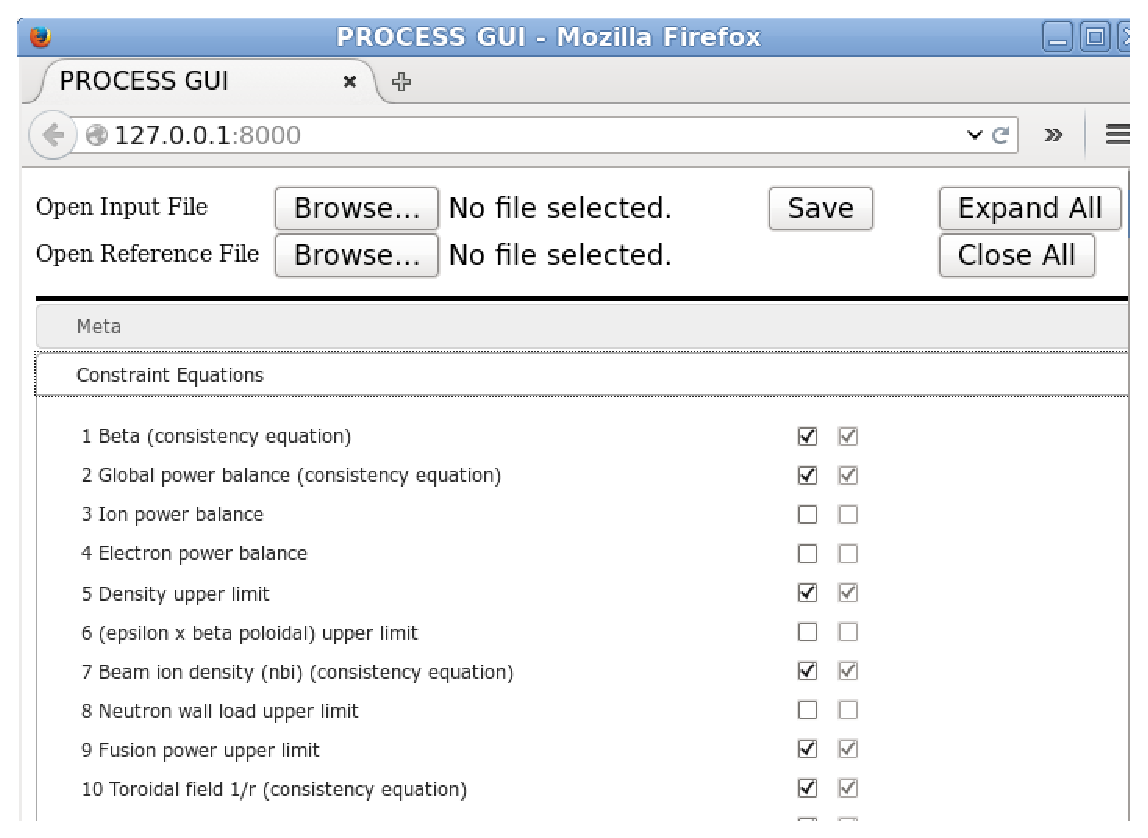
\includegraphics[scale=1]{gui.eps}

Every variable is listed along with its current value, a 'reference'
value and a short description. Hovering over the short description will
provide a longer description. Until an input file is opened, all values are given their default values assigned by \process. 

The reference values are used to compare differences between two files.
Differences between the reference value and the current input value will be
highlighted in red.

The 'Meta' section allows editing of the run description, which will be placed at the top of the created \indat. Iteration variables and constraint equations can be enabled using the checkboxes in the relevant sections.

An input file and a reference file can be opened using the buttons at the top
of the window. The files opened must be compatible with the \process\ version
number shown in the top right of the window.

The 'Save' button creates an \indat\ file with a similar layout to the GUI. Variables whose values are set different from the \process\ default are listed under module headings, along with a comment describing the variable. For integer variables, a description of the value
selected may also be included. The variables \texttt{neqns} (number of constraints) and \texttt{nvar} (number of iteration variables) are automatically calculated.

When using the Firefox web browser it can save time to select \\
\texttt{Preferences > General > Downloads > Always ask me where to save files.}

You can searching for a particular variable can be done using the browser's in-built search. Use the "Expand" button in the top-right of the window to expand every module heading and use Ctrl-f to search.

\section{Executing the Code}

Execute \process\ by simply typing \texttt{process} on the Unix command line.

By default, the input and output file names are as described in the following
sections. If, however, \process\ is executed with an argument, this is used as
a prefix to the file names:
\begin{quote}
\begin{verbatim}
process myrun
\end{verbatim}
\end{quote}
will assume that the input file is called \textit{myrun}\indat, etc.

The input file must be in the current directory.  The output files \textit{myrun}\outdat\
and \textit{myrun}\mfile\ will be created in the current directory.

\section{The Input File}
\label{sec:infile}

The input file \indat\ is used to change the values of the physics,
engineering and other code parameters from their default values, and to set up
the numerics (constraint equations, iteration variables etc.) required to
define the problem to be solved.  The user interface writes the input file, so
it is not necessary to edit it directly.  Details of layout and format are in
Appendix~\ref{app:infile}.

If the code encounters a problem reading the input file, it will stop
immediately with an error message. The last line of the output file \outdat\
may give an indication of where in the input file the problem lies.

\section{The Output Files}

The main output from the code is sent to file \outdat\ in the working
directory.  It is essential to check that the code reports that it has found a
\textit{feasible solution}.

A second file, \mfile, is also produced in the working directory.  This file
contains most of the same data as \outdat\ but in a different format, and has
been designed to be ``machine-readable'' by some of the utility programs
described in Chapter~\ref{chap:utilities}, to allow simple post-processing and
graphical output to be produced easily.

\section{Optimisation mode}

Switch \texttt{ioptimz} should be set to \texttt{1} for optimisation mode. 

If \texttt{ioptimz = 0}, a non-optimisation pass is performed first.  Occasionally this provides a feasible set of initial conditions that aids convergence of the optimiser, but it is recommended to use \texttt{ioptimz = 1}. 

Enable all the relevant consistency equations, and it is advisable to enable the corresponding iteration variables shown in bold in Table~\ref{tab:eqns}. A number of limit equations (inequality constraints) can also be activated.  For limit equations, the corresponding f-value must be selected as an iteration variable.  In optimisation mode, the number of iteration variables is unlimited.

It may still be difficult, if not impossible, to reconcile the fusion power
and the net electric power with the required values. This may well be due to
the power conversion efficiency values being used --- refer to
Figure~\ref{fig:powerflow3}.

With luck, a few iterations of this process will produce an adequate benchmark
case. A typical input file for use with \process\ in non-optimisation mode is
contained in Appendix~\ref{app:infile1}.

If scans of a given variable are to be made over a large range of
values, it is often a good idea to start the scan in the middle of the desired
range, and to split the scan in two --- one going downwards from the initial
value, and the other upwards.  This ensures that the whole range of the scan
produces well-converged machines (assuming a ``good'' initial point), without
sharp changes in gradient in the parameter values.

It should be remembered that the value of the scan variable is set in the
array \texttt{sweep}, and this overrules any value set for the variable
elsewhere in the input file. 

The output from an optimisation run contains an indication as to which iteration variables lie at their limiting values. A typical input file for use with \process\ in optimisation mode is contained in Appendix~\ref{app:infile2}.

\section{Non-optimisation mode}
\label{sec:optim}

Non-optimisation mode is sometimes used to perform benchmark comparisons, whereby the
machine size, output power etc.\ are known and one only wishes to find the
calculated stresses, beta values and fusion powers, for example. 

Running \process\ in non-optimisation mode requires few changes to be made to the
input file from the non-optimisation case. The main differences between
optimisation mode and non-optimisation mode are:

\begin{enumerate}

\item Non-optimisation mode does NOT apply lower or upper bounds to the iteration
  variables.  It follows that limit equations are not enforced.

\item In non-optimisation mode the number of active iteration variables must be equal to the number of constraints.

\item A figure of merit is not available in non-optimisation mode.

\item Scans cannot be performed in non-optimisation mode.

\end{enumerate}

As before, the user must decide which constraint equations and iteration
variables to activate. 


\section{Troubleshooting}
\label{sec:problems}

Experience has shown that the first few attempts at running \process\ with a
new input file tends to produce unfeasible results --- that is, the code will
not find a consistent set of machine parameters. The highly non-linear nature
of the numerics of \process\ is the reason for this difficulty, and it often
requires a great deal of painstaking adjustment of the input file to overcome.  The utility 
\texttt{a\_to\_b} (~\autoref{sec:atob}) is useful in this situation.

\subsection{Error handling}
\label{sec:errors}

In general, errors detected during a run are handled in a consistent manner,
with the code producing (hopefully) useful diagnostic messages to help the
user understand what has happened.

There are three levels of errors and warning that may occur:
\begin{description}

\item{Level 1:} An \textit{informational}\/ message is produced under certain
  conditions, for example if the code has modified the user's input choice for
  some reason.

\item{Level 2:} A \textit{warning}\/ message is produced if a non-fatal situation has
  occurred that may result in an output case that is inaccurate or
  unreliable in some way.

\item{Level 3:} An \textit{error}\/ message will occur if a severe or fatal
  error has occurred and the program cannot continue.

\end{description}

These messages are printed on the screen during the course of a run, and those
still active at the final (feasible or unfeasible) solution point are also
written to the end of the output file (messages encountered during the
iteration process are not copied to the output file, as the convergence to a
valid solution might resolve some of the warnings produced earlier in the
solution process).

The \texttt{error\_status} variable returns the highest severity level that
has been encountered (or zero if no abnormal conditions have been found); if a
severe error (level 3) is flagged at any point the program is terminated
immediately. The final message number encountered during a run is returned via
output variable \texttt{error\_id}. In addition, with certain messages, a
number of diagnostic values may also be given; these can be used to provide
extra diagnostic information if the source code is available.

\subsection{General problems}

A code of the size and complexity of \process\ contains myriads of equations
and variables. Virtually everything depends indirectly on everything else
because of the nature of the code structure, so perhaps it is not surprising
that it is often difficult to achieve a successful outcome.

Naturally, problems will occur if some of the parameters become unphysical.
For example, if the aspect ratio becomes less than or equal to one, then we
must expect problems to appear. For this reason, the bounds on the
iteration variables should be selected with care.

Occasionally arithmetic (``\texttt{NaN}'') errors are reported. They usually occur when the code is exploring unphysical values of the parameters, and often suggest that no feasible solution exists for the input file used.

The error messages produced by the code attempt to provide diagnostic
information, telling the user where the problem occurs, and also suggest a
possible solution. These messages are out of necessity brief, and so cannot
promise to lead to a more successful outcome.

There is the option to turn on extra debugging output; to do this, set \texttt{verbose = 1} in the input file.

\subsection{Optimisation problems}

On reflection it is perhaps surprising that \process\ ever does manage to
find the global minimum figure of merit value, since if there are
\texttt{nvar} iteration variables active the search is over
\texttt{nvar}-dimensional parameter space, in which there may be many shallow
minima of approximately equal depth. Remember that \texttt{nvar} is usually of
the order of twenty.

The machine found by \process\ may not, therefore, be the absolutely optimal
device. It is quite easy to have two or more solutions, with results only a
few per cent different, but a long way apart in parameter space. The technique
of ``stationary'' scans is sometimes used in this situation: a scan is requested, but the same value of the scan variable is listed repeatedly.

Scans should be started in the middle of a range of values, to try to keep the
scan within the same family of machines. The optimum machine found may
otherwise suddenly jump to a new region of parameter space, causing the output
variables to seem to vary unpredictably with the scanning variable.

It should be noted that in general the machine produced by \process\ will
always sit against one or more operation limits. If, during a scan, the limit
being leant upon changes (i.e.\ if the machine jumps from leaning on the beta
limit to leaning on the density limit) the output parameters may well become
discontinuous in gradient, and trends may suddenly change direction.

\subsection{Unfeasible results}

In the numerics section of the output file, the code indicates whether the run
produced a feasible or unfeasible result.

The former implies a successful outcome, although it is always worth checking
that the sum of the squares of the constraint residuals (\texttt{sqsumsq}) is small ($\sim
10^{-3}$ or less); the code will issue a warning if the solver reports convergence but
the value of \texttt{sqsumsq} exceeds $10^{-2}$. If this occurs, reducing the
value of the HYBRD tolerance \texttt{ftol} or \vmcon\ tolerance
\texttt{epsvmc} as appropriate should indicate whether the result is valid
or not; the output can usually be trusted if (1) the constraint
residues\footnote{The constraint residues are the final values of $c_i$ in the
  constraint equations --- see Section~\ref{sec:constraints}. The value
  \texttt{sqsumsq} is the square root of the sum of the squares of these
  residuals.} fall as the tolerance is reduced to about $10^{-8}$, and (2) the
code indicates that a feasible solution is still found.

An unfeasible result occurs if \process\ cannot find a set of values for the
iteration variables which satisfies all the given constraints. In this case,
the values of the constraint residues shown in the output give some indication
of which constraint equations are not being satisfied --- those with the
highest residues should be examined further. In optimisation mode, the code
also indicates which iteration variables lie at the edge of their allowed
range.

Unfeasible runs can be caused by specifying physically incompatible input parameters,  using insufficient iteration variables, or by starting the problem with unsuitable values of the iteration variables. 

The utility \texttt{run\_process} (Section~\ref{subsec:run_process}) carries out many runs, changing the starting values of the iteration variables randomly.  It stops once a feasible solution is found.

Another approach is to start with an input file that gives a feasible solution, and modify it step by step towards the parameters desired.  This process is automated by the 
utility \texttt{a\_to\_b} ((Section~\ref{sec:atob}).

It is important to choose the right number of \textit{useful}\/ iteration variables for the
problem to be solved --- it is possible to activate too many iteration variables as well as too few, some of which may be redundant.

Both optimisation and non-optimisation runs can fail with an error message
suggesting that the iteration process is not making good progress. This is
likely to be due to the code finding itself unable to escape a region of the
parameter space where the minimum in the residuals is significantly above
zero. In this situation, there is either no solution possible (the residuals
can therefore never approach zero), or the topology of the local minimum makes
it difficult for the code to escape to the global minimum. Again, a helpful
technique is to either change the list of iteration variables in use, or to
simply modify their initial values to try to help the code avoid such regions.

A technique that occasionally removes problems due to unfeasible results,
particularly if an error code \texttt{ifail = 3} is encountered during an
optimisation run, is to adjust slightly one of the limits imposed on the
iteration variables, even if the limit in question has not been reached. This
subtly alters the gradients computed by the code during the iteration process,
and may tip the balance so that the code decides that the device produced is
feasible after all. For instance, a certain component's temperature might be
400~K, and its maximum allowable temperature is 1000~K\@. Adjusting this limit
to 900~K (which will make no difference to the \textit{actual}\/ temperature)
may be enough to persuade the code that it has found a feasible solution.

Similarly, the order in which the constraint equations and iteration variables
are stored in the \texttt{icc} and \texttt{ixc} arrays can make the difference
between a feasible and unfeasible result. This seemingly illogical behaviour
is, sadly, typical of the way in which the code works.

Another technique in such situations may be to change the finite difference
step length \texttt{epsfcn}, as this might subtly change the path taken in the
approach towards a solution.

It may be the case that the act of satisfying all the required constraints is
impossible. No machine can exist if the allowed operating regime is too
restrictive, or if two constraint equations require conflicting
(non-overlapping) parameter spaces. In this case some relaxation of the
requirements is needed for the code to produce a successful machine design.

\subsection{Hints}

The above sections should indicate that it is the complex interplay between
the constraint equations and the iteration variables that determines whether
the code will be successful at producing a useful result. It can be a somewhat
laborious process to arrive at a working case, and (unfortunately, perhaps)
experience is often of great value in this situation.

It should be remembered that sufficient iteration variables should be used to
solve each constraint equation. For instance, a particular limit equation may
be $A \leq B$, i.e.\ $A = fB$, where the f-value $f$ must lie between zero and
one for the relation to be satisfied.  However, if none of the iteration
variables have any effect on the values of $A$ and $B$, and $A$ happens to be
\textit{greater}\/ than $B$, then \process\ will clearly not be able to solve
the constraint.

The lower and upper bounds of the iteration variables are all available to be
changed in the input file. Constraints can be relaxed in a controlled manner
by moving these bounds, although in some cases care should be taken to ensure
that unphysical values cannot occur.  The code indicates which iteration
variables lie at the edge of their range.

It is suggested that constraint equations should be added one at a time, with
sufficient new iteration variables activated at each step.  If the situation
becomes unfeasible it can be helpful to reset the initial iteration variable
values to those shown in the output from a previous feasible case, and rerun
the code.

